\documentclass[twocolumn]{extarticle}
\usepackage{fontspec}   %加這個就可以設定字體
\usepackage{xeCJK}       %讓中英文字體分開設置
\usepackage{indentfirst}
\usepackage{listings}
\usepackage[newfloat]{minted}
\usepackage{float}
\usepackage{graphicx}
\usepackage{caption}
\usepackage{fancyhdr}
\usepackage{hyperref}
\usepackage{amsmath}
\usepackage{multirow}
\usepackage[dvipsnames]{xcolor}
\usepackage{graphicx}
\usepackage{tabularx}
\usepackage{booktabs}
\usepackage{caption}
\usepackage{subcaption}
\usepackage{pifont}
\usepackage{amssymb}
\usepackage{titling}

\usepackage{pdftexcmds}
\usepackage{catchfile}
\usepackage{ifluatex}
\usepackage{ifplatform}

\usepackage[breakable, listings, skins, minted]{tcolorbox}
\usepackage{etoolbox}
\setminted{fontsize=\footnotesize}
\renewtcblisting{minted}{%
    listing engine=minted,
    minted language=verilog,
    listing only,
    breakable,
    enhanced,
    minted options = {
        linenos, 
        breaklines=true, 
        breakbefore=., 
        % fontsize=\footnotesize, 
        numbersep=2mm
    },
    overlay={%
        \begin{tcbclipinterior}
            \fill[gray!25] (frame.south west) rectangle ([xshift=4mm]frame.north west);
        \end{tcbclipinterior}
    }   
}

\usepackage[
top=1.5cm,
bottom=0.75cm,
left=1.5cm,
right=1.5cm,
includehead,includefoot,
heightrounded, % to avoid spurious underfull messages
]{geometry} 

\newenvironment{code}{\captionsetup{type=listing}}{}
\SetupFloatingEnvironment{listing}{name=Code}
\usepackage[moderate]{savetrees}


\title{Computer Organization HW3}
\author{110550088 李杰穎}
\date{\today}


\setCJKmainfont{Noto Serif TC}


\ifwindows
\setmonofont[Mapping=tex-text]{Consolas}
\fi

\XeTeXlinebreaklocale "zh"             %這兩行一定要加,中文才能自動換行
\XeTeXlinebreakskip = 0pt plus 1pt     %這兩行一定要加,中文才能自動換行

\setlength{\parindent}{0em}
\setlength{\parskip}{1em}
\renewcommand{\baselinestretch}{1.25}
\setlength{\droptitle}{-7.5em}   % This is your set screw
\setlength{\columnsep}{2em}

\begin{document}

\maketitle

\section{Architecture Diagrams}

本次作業的架構圖與 spec 相同,可參照 \autoref{fig:arch}。比較特別的是 ALU Control 輸出的 \texttt{leftRight} 實際上是 \texttt{ALU\_operation[3]}。

\begin{figure}[htbp]
\centering
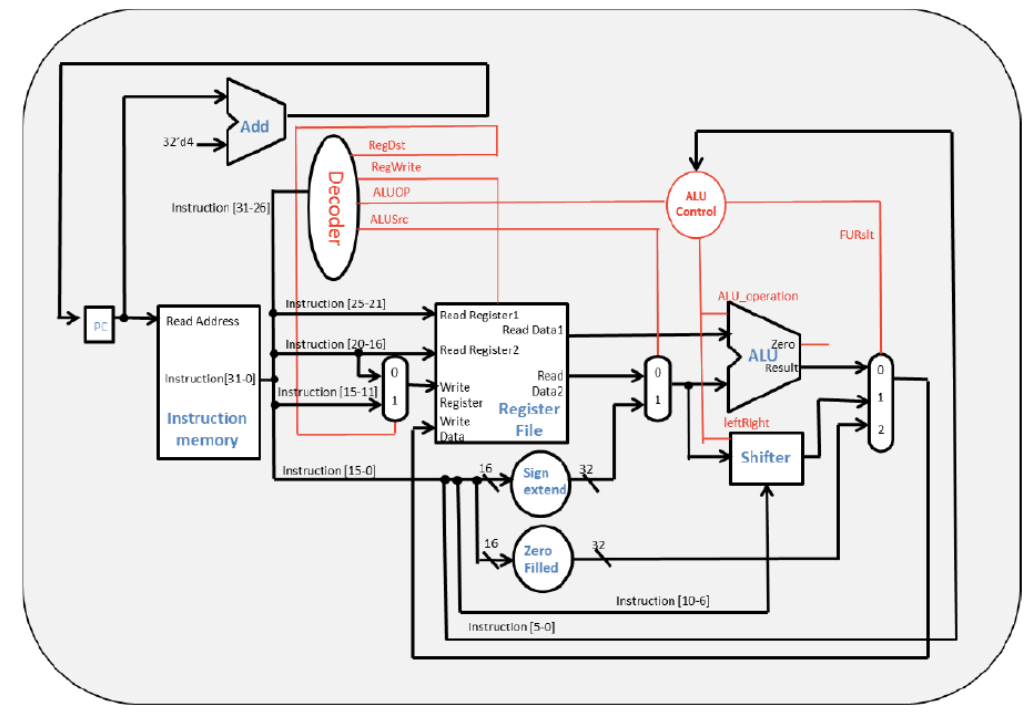
\includegraphics[width=0.95\linewidth]{arch}
\caption{本次作業的整體架構圖}
\label{fig:arch}
\end{figure}

\section{Hardware Module Analysis}

本次作業共需要完成以下 11 個 modules:

\begin{enumerate}
\item \texttt{Adder}
\item \texttt{Mux2to1}
\item \texttt{Mux3to1}
\item \texttt{ALU\_1bit}
\item \texttt{ALU}
\item \texttt{Shifter}
\item \texttt{Sign\_Extend}
\item \texttt{Zero\_Filled}
\item \texttt{ALU\_Ctrl}
\item \texttt{Decoder}
\item \texttt{Simple\_Single\_CPU}
\end{enumerate}

接下來會介紹每個 module 的功能及實作細節。

\subsection{\texttt{Adder}}

此 module 功能為相加兩個 32 bit 的數字,故實作細節相當簡單。即利用 \texttt{assign} 去將相加後的結果 assign 到 output wire 上。

\subsection{\texttt{Mux2to1}}

此 module 為一個 2 to 1 MUX,利用一個 1 bit 的 select 去選擇輸出的數值是哪一個輸入。值得注意的是,此 module 使用 \texttt{parameter size} 去控制輸入及輸出位元的數量。 

實作主要是利用三元運算子去進行類似於 if-else 的輸出控制。

\subsection{\texttt{Mux3to1}}

此 module 為一個 3 to 1 MUX,利用一個 2 bit 的 select 去選擇輸出的數值是哪一個輸入。其餘細節皆與 \texttt{Mux2to1} 類似。

\subsection{\texttt{ALU\_1bit}}

本 module 是使用前次作業的程式碼,主要就是根據 \texttt{operation, invertA, invertB, carryIn, less} 去輸出 1 bit 的 ALU 計算結果。實作細節就不再贅述。

\subsection{\texttt{ALU}}

本 module 是利用 32 個 \texttt{ALU\_1bit} module 去計算 32 bit 的 ALU 結果,值得注意的是最低位元 bit 的 \texttt{set} input 是最高位元 ALU 中加法器的計算結果。且為了讓中間 30 個 ALU 可以更簡單的被產生,使用了 \texttt{generate, for} 去重複產生 1-bit ALU module。

\subsection{\texttt{Shifter}}

本 module 為輸入一 32 bit 的數字,將其根據 \texttt{shamt, leftRight},進行左移或右移的操作。實作細節就是同樣利用三元運算子去進行 \texttt{leftRight} 的判斷,再利用 \texttt{<<, >>} 兩個 operator 去進行左移和右移的操作。值得注意的是因為我們是實作 \texttt{sll, srl} 這兩個 instruction,所以我們並不需要根據最高位元去進行補 1 或 0 的判斷。

\subsection{\texttt{Sign\_Extend}}

本 module 為輸入一 16 bit 的數字,利用其最高位元判斷正負性,再將其 extend 成 32 bit 的數字。這邊主要的細節是利用 \texttt{\{16\{data\_i[15]\}\}} 這個語法去做到對於最高的 16 bits 填入第 16 bit 的值。

\subsection{\texttt{Zero\_Filled}}

本 module 在此次作業並沒有用到,但其功能與 \texttt{Sign\_Extend} 類似,都是將 16 bit 的數字擴展到 32 bit,不同的是本 module 不會根據 16 bit 的最高位判斷最高的 16 bit 要填上 1 或是 0,而是統一填上 0。


\subsection{\texttt{Decoder}}

本 module 是根據 instruction 中的最高 6 bit 的 \texttt{opcode},輸出用於控制 ALU 的 \texttt{ALUOp} 訊號、控制 ALU 輸入的 \texttt{ALUSrc}、控制 register memory 是否啟用寫入的 \texttt{RegWrite} 及寫入 register 的 address \texttt{RegDst}。

\subsection{\texttt{ALU\_Ctrl}}

本 module 會根據 \texttt{Decoder} 的輸出,\texttt{ALUOp} 及 instruction 最低的 6 bit,也就是 \texttt{funct} 生成用於控制 ALU 的 \texttt{ALU\_operation} 及控制 write data 的輸入的 MUX 的 select \texttt{FURSlt}。

實作部分也是利用三元運算子,根據 \texttt{ALU\_operation} 及 \texttt{funct} 去計算出正確的輸出。

\subsection{\texttt{Simple\_Single\_CPU}}

本 module 為本次作業的核心 module, 其將以上的 module 組合起來,構造出本次作業要求的 Simple Single Cycle CPU。實作細節與 spec 中描述的相同,基本上就是生成出不同的 wire,再將 wire 連接到正確的 module 上。


\section{Finished Part}

本次作業我完成了所有需要完成的 module,並也通過助教提供的三個測資。

\section{Problems and Solutions}

在第一次接完線之後,發現並不能輸出正確的答案,且輸出的結果為 $\times$。利用在 test bench 中增加 \texttt{\$display} 進行 debug 後發現問題出在 ALU 中,最後才發現原來是在將 \texttt{ALU\_operation\_i} 分解出 \texttt{invertA}、\texttt{invertB} 及 \texttt{operation} 時,錯誤的將 wire 取名為 \texttt{invert\_A},導致無法執行出正確的結果,導致最終結果變成 $\times$。

\section{Summary}

在本次作業中,我完成了簡單的 Single Cycle CPU,此 CPU 僅支援有限的 ISA,如 MIPS 中的 \texttt{lw, sw, beq} 等 instruction 都尚不能在本次實作的 CPU 中使用,且本次作業的 CPU 也沒有加上 Data Memory,這也使得支援的指令有一定的受限。但是在本次作業中,我還是大致理解 CPU 的實作流程,並能夠正確的使用 verilog 實作出可以正確運作的 CPU。

\end{document}